% !TEX root = ../dg.tex

\section{Geodesics on Lie Groups}
\label{sec:geodesics on lie groups}

In \Cref{sec:geodesics} we defined geodesics as the curves $\gamma \from I \to M$ with $\frac{D\gamma'}{dt} = 0$, which means that geodesics are parametrized at constant speed and are straight (in the sense that they don't turn). Compare to the fact that straight lines $\alpha \from I \to \R^n$ traversed at constant speed satisfy $\alpha''(t)= 0$.

It seems intuitively obvious that the shortest path between two points should be as straight as possible, and hence should be a geodesic. Of course, we have to be careful because there is generally not a \emph{unique} geodesic between two points (think about points on the sphere) and there may be no geodesic at all (think about the points $(2,0)$ and $(-2,0)$ in the annulus $\{(x,y) \in \R^2 : 1 < x^2 + y^2 < 4\}$). But if two points are close enough, there will be a unique minimizing geodesic between them.

But, from \Cref{thm:exp is a local diffeo}, we know that for any $p \in M$ there exists $\epsilon > 0$ so that $\exp_p \from B_\epsilon(0) \to M$ is a diffeomorphism. The image $\exp_p(B_\epsilon(0))$ is called a \emph{normal ball} or \emph{geodesic ball} of radius $\epsilon$ around $p$, and denoted $B_\epsilon(p)$.

\begin{theorem}\label{thm:locally minimality of geodesics}
	Within any normal ball $B_\epsilon(p)$, the geodesic rays from $p$ are the unique shortest paths from $p$ to their endpoints.
\end{theorem}

The proof of this theorem is fairly technical and not very enlightening, so we skip it. For details, see do Carmo~\cite[\S 3.3]{docarmoRiemannianGeometry1992}.

Instead, let's go a bit deeper on geodesics on Lie groups.

\subsection{Bi-Invariant Metrics}

First of all, recall from \Cref{ex:left-invariant metrics} that we can define a left-invariant Riemannian metric on any Lie group $G$ by choosing an inner product $\langle \cdot , \cdot \langle$ on $T_eG \cong \mathfrak{g}$, and then pulling it back to each tangent space: for $h \in G$ and $u,v \in T_hG$,
\begin{equation}\label{eq:left-invariant metric def}
	g_h(u,v) := \langle (dL_{h^{-1}})_h u, (dL_{h^{-1}})_hv \rangle_e,
\end{equation}
and similarly we could have gotten a right-invariant metric using $R_{h^{-1}}$ rather than $L_{h^{-1}}$.

Formally, we define a \emph{left-invariant Riemannian metric} on $G$ by requiring that
\[
	g_{h_1}(u,v) = g_{h_2h_1}((dL_{h_2})_{h_1}u, (dL_{h_2})_{h_1}v)
\]
for each $h_1,h_2 \in G$ and each $u,v \in T_{h_1}G$. Note that $(dL_{h_2})_{h_1} \from T_{h_1}G \to T_{L_{h_2}(h_1)}G = T_{h_2h_1}G$, so the right-hand side makes sense.

In other words, a metric is left-invariant if all left translations are isometries of $G$.

\begin{exercise}
	Show that the metric $g$ defined by \eqref{eq:left-invariant metric def} is left-invariant in the above sense.
\end{exercise}

Similarly, we say that a metric on $G$ is \emph{right-invariant} if all right translations are isometries. 

In general, there are lots of left-invariant metrics on a Lie group, and also lots of right-invariant metrics. And it's not so clear which one to pick, or even whether to pick a left-invariant one or a right-invariant one. 

However, in certain special cases we get Riemannian metrics on Lie groups which are both left-invariant and right-invariant. We call such metrics \emph{bi-invariant} and they are, in some sense, the best possible Riemannian metrics to put on Lie groups: they are highly symmetric, and we don't have to choose whether we prefer left- or right-invariance. Moreover, under appropriate hypotheses, bi-invariant metrics are essentially unique; see \Cref{thm:uniqueness of bi-invariant metrics}.

Note that left/right/bi-invariant metrics on $G$ are completely determined by the inner product
\[
	\langle \cdot , \cdot \rangle_e = g_e(\cdot , \cdot)
\]
on $T_eG \cong \mathfrak{g}$; after all, any metric on $G$ determines such an inner product, and such an inner product uniquely determines a left-invariant metric using \eqref{eq:left-invariant metric def} (or a right-invariant metric using the analogous formula replacing $L_{h^{-1}}$ with $R_{h^{-1}}$; if the two agree, then what either gives is a bi-invariant metric).

\begin{proposition}\label{prop:characterization of bi-invariant metric}
	Suppose the Lie group $G$ admits a bi-invariant metric. Then the induced inner product on $\mathfrak{g}$ satisfies
	\[
		\langle [X,Y],Z\rangle_e = \langle Y, [Z,X]\rangle_e
	\]
	for all $X,Y,Z \in \mathfrak{g}$.
\end{proposition}

\begin{proof}
	Since $X,Y,Z \in \mathfrak{g}$, they are (or can be identified with) left-invariant vector fields on $G$. Let $\Phi_t$ be the local flow associated to $X$. Because the metric is bi-invariant we know that
	\begin{align*}
		\langle Y, Z \rangle_e = g_e(Y,Z) & = g_e \left( (dR_{\Phi_t(e)})_{\Phi_t^{-1}(e)}(dL_{\Phi_t^{-1}(e)} )_e Y_e, (dR_{\Phi_t(e)})_{\Phi_t^{-1}(e)}(dL_{\Phi_t^{-1}(e) })_e Z_e\right) \\
		& = g_e \left( (dR_{\Phi_t(e)})_{\Phi_t^{-1}(e)} Y_{\Phi_t^{-1}(e)}, (dR_{\Phi_t(e)})_{\Phi_t^{-1}(e)} Z_{\Phi_t^{-1}(e)}\right) \\
		& = \langle (dR_{\Phi_t(e)})_{\Phi_t^{-1}(e)} Y_{\Phi_t^{-1}(e)}, (dR_{\Phi_t(e)})_{\Phi_t^{-1}(e)} Z_{\Phi_t^{-1}(e)} \rangle_e
	\end{align*}
	by left-invariance of $Y$ and $Z$. 
	
	Differentiating the above expression with respect to $t$, evaluating at $t=0$, and recalling that the Lie bracket is the same as the Lie derivative eventually yields
	\[
		0 = \langle [Y,X],Z \rangle_e + \langle Y, [Z,X] \rangle,
	\]
	which is equivalent to the stated equation.
\end{proof}

If we set $X=Z$ in \Cref{prop:characterization of bi-invariant metric}, then we see that
\[
	\langle [X,Y],X \rangle_e = 0.
\]
In other words:
\begin{corollary}\label{cor:bracket orthogonal}
	In a bi-invariant metric, the bracket of two left-invariant vector fields $X$ and $Y$ is orthogonal to both $X$ and $Y$. 
\end{corollary}

In fact, the converse of \Cref{prop:characterization of bi-invariant metric} is also true, so we get the following characterization of bi-invariant metrics on Lie groups:

\begin{theorem}\label{thm:bi-invariant metric condition}
	A Riemannian metric on a Lie group $G$ is bi-invariant if and only if the induced inner product on $\mathfrak{g}$ satisfies
	\[
		\langle [X,Y],Z\rangle_e = \langle Y, [Z,X]\rangle_e
	\]
	for all $X,Y,Z \in \mathfrak{g}$.
\end{theorem}


\begin{example}\label{ex:no bi-invariant metric on aff}
	The goal here is to show that $\Aff^+(\R)$ does \emph{not} admit a bi-invariant metric. Recall from \Cref{ex:coords on affine group} that we have left-invariant vector fields $A,B \in \mathfrak{aff}^+(\R)$ with $[A,B]=B$. If $\Aff^+(\R)$ admits a bi-invariant metric, then \Cref{prop:characterization of bi-invariant metric} (or \Cref{thm:bi-invariant metric condition}) implies that the induced inner product on $\mathfrak{aff}^+(\R) \cong \R^2$ satisfies
	\[
		0 = \langle [B,B],A \rangle_e = \langle B, [B,A] \rangle_e = \langle B, -B\rangle_e = -\langle B,B\rangle_e \neq 0
	\]
	since $B$ is not the zero vector and the inner product must be positive-definite. So there is no such bi-invariant metric.
\end{example}

It is a bit unfortunate that not all Lie groups admit bi-invariant metrics, but it turns out that all \emph{compact} Lie groups do. In service of proving this, let's first record the following observation:

\begin{lemma}\label{lem:bi-invariant metrics conjugation invariant}
	A Lie group $G$ admits a bi-invariant Riemannian metric if and only if there is an inner product on $T_eG$ which is invariant under conjugation.
\end{lemma}

\begin{proof}
	($\Rightarrow$) For the forward direction, suppose $G$ has a bi-invariant metric $g$. Let $\langle \cdot , \cdot \rangle_e$ be the induced inner product on $T_eG$, and observe that, for any $h \in G$ and any $X,Y \in \mathfrak{g}$,
	\begin{multline*}
		\langle (dC_h)_e X_e, (dC_h)_e Y_e \rangle_e = \langle d(L_h \circ R_{h^{-1}})_e X_e, d(L_h \circ R_{h^{-1}})_e Y_e \rangle_e = \langle (dL_h)_{h^{-1}} (dR_{h^{-1}})_e X_e, (dL_h)_{h^{-1}} (dR_{h^{-1}})_e Y_e \rangle_e \\
		= g_{h^{-1}} ((dR_{h^{-1}})_e X_e,(dR_{h^{-1}})_e Y_e) = g_e(X_e,Y_e) = \langle X_e, Y_e \rangle_e
	\end{multline*}
	by left- and right-invariance of $g$. So $\langle \cdot , \cdot \rangle_e$ is conjugation-invariant.
	
	($\Leftarrow$) On the other hand, suppose $\langle \cdot , \cdot \rangle_e$ is conjugation-invariant. Define the left-invariant metric $g$ by \eqref{eq:left-invariant metric def}. I claim that $g$ is also right-invariant, and hence bi-invariant. To see this, let $h_1,h_2 \in G$. Notice that, for any $k \in G$,
	\[
		(L_{(h_1h_2)^{-1}} \circ R_{h_2})(k) = h_2^{-1}h_1^{-1}kh_2 = C_{h_2^{-1}}(L_{h_1^{-1}}(k)) = (C_{h_2^{-1}} \circ L_{h_1^{-1}})(k),
	\]
	and hence $L_{(h_1h_2)^{-1}} \circ R_{h_1} = C_{h_2^{-1}} \circ L_{h_1^{-1}}$.
	
	Therefore, for any vector fields $u,v \in T_{h_1}G$,
	\begin{align*}
		g_{h_1h_2}((dR_{h_2})_{h_1}u, (dR_{h_2})_{h_1}v) & = \langle (dL_{(h_1h_2)^{-1}})_{h_1h_2}(dR_{h_2})_{h_1}u, (dL_{(h_1h_2)^{-1}})_{h_1h_2}(dR_{h_2})_{h_1}v \rangle_e \\
		& = \langle (d(L_{(h_1h_2)^{-1}}\circ R_{h_2})_{h_1}u, (d(L_{(h_1h_2)^{-1}}\circ R_{h_2})_{h_1}v \rangle_e \\
		& = \langle (d(C_{h_2^{-1}} \circ L_{h_1^{-1}})_{h_1}u, (d(C_{h_2^{-1}} \circ L_{h_1^{-1}})_{h_1}v \rangle_e \\
		& = \langle (dC_{h_2^{-1}})_{e} (dL_{h_1^{-1}})_{h_1}u, (dC_{h_2^{-1}})_{e} (dL_{h_1^{-1}})_{h_1}v \rangle_e
	\end{align*}
	by the chain rule. But now conjugation-invariance of $\langle \cdot , \cdot \rangle_e$ implies this is equal to
	\[
		\langle (dL_{h_1^{-1}})_{h_1}u, (dL_{h_1^{-1}})_{h_1}v \rangle_e = g_{h_1}(u,v)
	\]
	by definition of $g$. Stringing these equalities together gives 
	\[
		g_{h_1h_2}((dR_{h_2})_{h_1}u, (dR_{h_2})_{h_1}v) = g_{h_1}(u,v),
	\]
	which is the definition of right-invariance. So we see that the left-invariant metric $g$ is also right-invariant, and hence it is bi-invariant.
\end{proof}

We're now ready to show that all \emph{compact} Lie groups admit a bi-invariant metric. The strategy is to pick any arbitrary inner produce on $T_eG$ and then average it over all conjugations. If the group is non-compact, then this could easily fail: the averaging procedure might fail to converge. But when $G$ is compact, this isn't a problem:

\begin{theorem}\label{thm:bi-invariant metrics}
	Every compact Lie group $G$ admits a bi-invariant Riemannian metric.
\end{theorem}

\begin{proof}
	Start with a right-invariant metric on $G$, and let $\dVol \in \Omega^n(G)$ be the associated right-invariant volume form guaranteed by \Cref{def:Riemannian volume form}. That is, $\dVol(h) \in \bigwedge^n(T_hG)^\ast$ for all $h \in G$.
	
	Now, let $\langle \cdot , \cdot \rangle_e$ be an arbitrary inner product on $T_eG$. Then we define a new inner product $\langle \cdot , \cdot \rangle_e'$ by averaging over conjugations:
	\[
		\langle u, v \rangle_e' := \int_{h \in G} \langle (dC_h)_e u, (dC_h)_ev \rangle_e \dVol(h).
	\]
	Here's where we using compactness, which guarantees that this integral converges. Right-invariance of the volume form now implies that
	\begin{align*}
		\langle (dC_{h_1})_e u, (dC_{h_1})_e v \rangle_e' & = \int_G \langle (dC_{h_2})_e (dC_{h_1})_e u, (dC_{h_2})_e (dC_{h_1})_e v \rangle_e \dVol(h_2) \\
		& =  \int_G \langle d(C_{h_2} \circ C_{h_1})_e u, d(C_{h_2} \circ C_{h_1})_e v \rangle_e \dVol(h_2) \\
		& =  \int_G \langle d(C_{h_2h_1})_e u, d(C_{h_2h_1})_e v \rangle_e \dVol(h_2) \\
		& =  \int_G \langle d(C_{h_2h_1})_e u, d(C_{h_2h_1})_e v \rangle_e R_{h_1}^\ast \dVol(h_2) \\
		& = \int_G \langle d(C_{h_2h_1})_e u, d(C_{h_2h_1})_e v \rangle_e \dVol(h_2h_1) \\
		& = \int_G \langle d(C_{h})_e u, d(C_{h})_e v \rangle_e \dVol(h) \\
		& = \langle u, v \rangle_e'
	\end{align*}
	using the change of variables formula for the map $R_{h_1} \from G \to G$, the right-invariance of $\dVol$, and then making the substitution $h= h_2h_1$.
	
	Therefore, $\langle \cdot , \cdot \rangle_e'$ is conjugation-invariant, and hence corresponds to a bi-invariant metric on $G$ by \Cref{lem:bi-invariant metrics conjugation invariant}.
\end{proof}

When $G$ is simple, the bi-invariant metric we get is essentially unique:

\begin{theorem}[{see, e.g.,~\cite[Proposition~2.48]{alexandrinoLieGroupsGeometric2015}}]\label{thm:uniqueness of bi-invariant metrics}
	Let $G$ be a compact, simple Lie group. Then the bi-invariant metric on $G$ is unique up to re-scaling.
\end{theorem}

\subsection{Geodesics in the Bi-Invariant Metric}

Recall that we defined an exponential map $\exp \from \mathfrak{g} \cong T_e G \to G$ for Lie groups in \Cref{sec:exponential map}. We also defined a \emph{Riemannian} exponential map $\exp_e \from T_e G \to G$ in \Cref{def:Riemannian exponential}. Of course, the Riemannian exponential depends on a choice of Riemannian metric, whereas the Lie group exponential map only depends on the Lie group structure. However, when we have a bi-invariant metric, the two exponential maps will agree, which is the main point of this section.

\begin{example}
	Recall our left-invariant metric on $\Aff^+(\R) \cong H$ from \Cref{ex:affine hyperbolic metric}. We saw in \Cref{ex:affine geodesics} that the geodesics for this metric are vertical lines and semi-circles centered at points on the $x$-axis. Therefore, the geodesics through the identity $(0,1)$ are as depicted in \Cref{fig:identity geodesics in aff}.
	
	\begin{figure}[htbp]
		\centering
			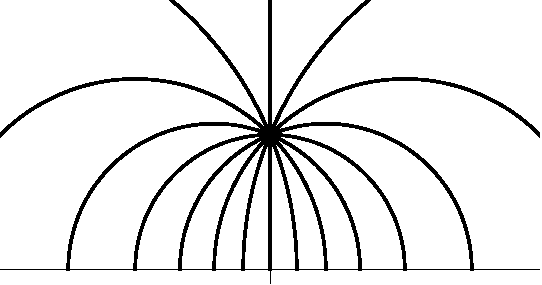
\includegraphics[height=1.5in]{affgeo.pdf}
		\caption{The geodesics through the identity in $\Aff^+(\R) \cong H$.}
		\alttext{Several geodesics in $H$ through $(0,1)$. One is the $y$-axis, the rest are semi-circles centered on the $x$-axis.}
		\label{fig:identity geodesics in aff}
	\end{figure}

	\ifplastex
	\begin{figure}[htbp]
		\centering
			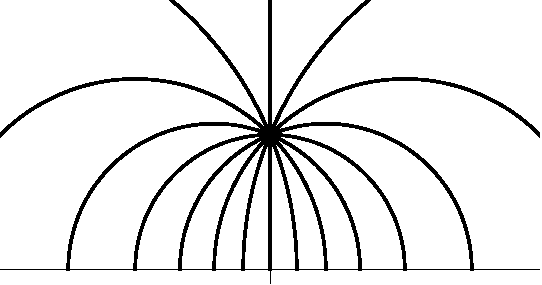
\includegraphics[height=1.5in]{affgeo.gif}
		\caption{An animation showing the family of geodesics through $(0,1)$.}
		\alttext{A continuous deformation between the geodesics from the previous figure.}
		\label{fig:identity geodesics in aff animation}
	\end{figure}
	\fi
	
	On the other hand, suppose $v = a \frac{\partial}{\partial x} + b \frac{\partial}{\partial y} \in T_{(0,1)}H$ is a tangent vector at the identity. Under the identification of $\Aff^+(\R)$ with the matrix group $\left\{\begin{bmatrix} y & x \\ 0 & 1 \end{bmatrix} : (x,y) \in \R^2, y > 0\right\}$ from \Cref{ex:affine group}, $v$ is identified with the $2 \times 2$ matrix
	\[
		A_v = \begin{bmatrix} b & a \\ 0 & 0 \end{bmatrix} \in T_I \GL_2(\R).
	\]
	In this setting, the exponential map is just the matrix exponential, so 
	\[
		\exp(tv) = I + tA_v + \frac{1}{2!} (tA_v)^2 + \dots = \begin{bmatrix} 1 & 0 \\ 0 & 1 \end{bmatrix} + t\begin{bmatrix} b & a \\ 0 & 0 \end{bmatrix} + \frac{t^2}{2!} \begin{bmatrix} b^2 & ab \\ 0 & 0 \end{bmatrix} + \frac{t^3}{3!} \begin{bmatrix} b^3 & ab^2 \\ 0 & 0 \end{bmatrix} + \dots = \begin{bmatrix} e^{tb} & \frac{a(e^{tb}-1)}{b} \\ 0 & 1 \end{bmatrix}.
	\]
	In other words, the one-parameter subgroup associated to $v \in T_{(0,1)}H$ is the curve $t \mapsto \left(\frac{a(e^{tb}-1)}{b},e^{tb}\right)$, as depicted in \Cref{fig:aff1par}.
	
	\begin{figure}[htbp]
		\centering
			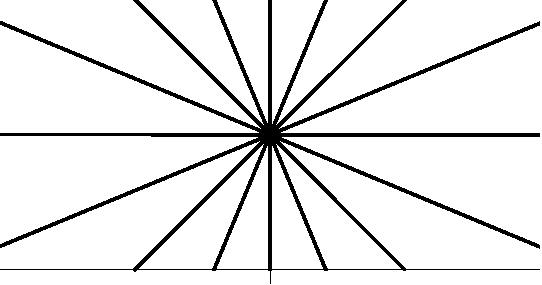
\includegraphics[height=1.5in]{aff1par}
		\caption{The one-parameter subgroups in $H$.}
		\alttext{The one-parameter subgroups, which are just the straight lines through the point $(0,1)$.}
		\label{fig:aff1par}
	\end{figure}
	
	Clearly, the one-parameter subgroups are \emph{not} geodesics with respect to the metric. The issue is, as we've already seen in \Cref{ex:no bi-invariant metric on aff}, that $\Aff^+(\R)$ does not have a bi-invariant metric.
\end{example}


\begin{theorem}\label{thm:bi-invariant exp}
	In a bi-invariant metric on a Lie group, the one-parameter subgroups coincide with the geodesics through the identity.
\end{theorem}

\begin{proof}
	Recall from \eqref{eq:levi-civita formula} the formula 
	\begin{equation*}
		g(\nabla_VU,W) = \frac{1}{2}\left[U(g(V,W)) + V(g(W,U)) - W(g(U,V)) - g([U,W],V) - g([V,W],U) - g([U,V],W)\right],
	\end{equation*}
	Assume $V,W \in \mathfrak{aff}^+(\R)$ are left-invariant, and let $U=V$ in the above equation. Since the metric is bi-invariant, $g(V,W)$ and $g(V,V)$ are constant, so the first three terms all vanish. The last term also vanishes since $[V,V]=0$, so we're left with
	\[
		g(\nabla_VV,W) = \frac{1}{2}\left[- g([V,W],V) - g([V,W],V)\right] = -g([V,W],V) = g([W,V],V) = 0
	\]
	by \Cref{cor:bracket orthogonal}.
	
	Since $W$ could have been any left-invariant vector field, this implies that $\nabla_VV = 0$ for all left-invariant vector fields $V$, where $\nabla$ is the Levi-Civita connection. But then if $\gamma(t) = \exp(tV_e)$ is the one-parameter subgoup associated with $V_e \in T_eG$, we have that
	\[
		\gamma'(t) = \frac{d}{dt} \exp(tV_e) = (d L_{\exp(tV_e)})_e V_e = V_{\exp(tV_e)},
	\]
	so $V$ is precisely the velocity field of the curve $\gamma$, and hence
	\[
		0 = \nabla_VV = \nabla_{\gamma'(t)} \gamma'(t) = \frac{D\gamma'}{dt}
	\]
	implies that $\gamma$ is a geodesic.
\end{proof}

Since the Lie group exponential is defined in terms of one-parameter subgroups and the Riemannian exponential is defined in terms of geodesics, \Cref{thm:bi-invariant exp} implies that the Lie group exponential and the Riemannian exponential are the same on a Lie group with a bi-invariant metric.


In particular, this means that on matrix groups with a bi-invariant metric we can often solve the following problem: given $h_1, h_2 \in G$, what is the minimizing geodesic from $h_1$ to $h_2$. To do so, note that it suffices to find a geodesic $\gamma(t)$ from the identity element $e$ to $h_1^{-1}h_2$: since left-multiplication is an isometry, $\alpha(t) = h_1 \gamma(t)$ will be a geodesic from $h_1$ to $h_2$. 

So we've reduced to finding the geodesic from the identity to any group element $h$. By \Cref{thm:bi-invariant exp}, this geodesic will be a one-parameter subgroup passing through $h$, so our goal is to find, say, a unit vector $v \in T_e G$ so that $\exp(t_0v) = h$. Then the curve $\gamma \from [0,t_0] \to G$ given by $\gamma(t) = \exp(tv)$ will be such a geodesic, and it will have length $t_0$. 

But inverting the matrix exponential is exactly what the matrix logarithm does. In general, since the log is multivalued, $\log(h)$ will be a collection of elements of $T_eG$, but if we choose $u$ with smallest norm and let $v = \frac{u}{\|u\|}$ then it will follow that $d(e,h) = \|u\|$ and $\gamma(t) = \exp(tv)$ is a minimizing geodesic from $e$ to $h$.

\begin{example}
	Consider $G = \SO(3)$. If $A \im \SO(3)$, then $A$ is unitarily diagonalizable:
	\[
		A = U D U^\ast,
	\]
	where $U \in \U(3)$ and $D = \diag(1,e^{i\theta},e^{-i\theta})$ is the diagonal matrix with eigenvalues of $A$ on the diagonal. Then
	\[
		\log(A) = U \log(D) U^\ast = U \diag(0,i\theta,-i\theta) U^\ast.
	\]
	So then the distance from $I$ to $A$ is
	\[
		\|\log(A)\| = \sqrt{2}\theta
	\]
	and the unit-speed geodesic from $I$ to $A$ is
	\[
		\gamma(t) = U \diag(1,e^{it/\sqrt{2}},e^{-it/\sqrt{2}}) U^\ast,
	\]
	with $A = \gamma(\sqrt{2}\theta)$.
	
	Of course, the same sort of thing works on $\SO(n)$ for any $n$.
\end{example}


%
% The key technical tool we will use is Gauss's Lemma, stated below as \Cref{lem:gauss}. To make sense of it, we need to talk about parametrized surfaces in manifolds:
%
% \begin{definition}\label{def:parametrized surface}
% 	Let $A \subset \R^2$ be an open set whose boundary $\partial A$ is a piecewise differentiable curve. A \emph{parametrized surface} in $M$ is a smooth mapping $s \from A \to M$. A \emph{vector field} $V$ along $s$ is a smooth mapping with $V(q) \in T_{s(q)}M$ for all $q \in A$.
% \end{definition}
%
% We can talk about coordinate curves in a parametrized surface $s$ as follows: for fixed $v_0 \in R$ and $u \in \R$ so that $(u,v_0) \in A \cap \{v = v_0\}$, we get a curve $u \mapsto s(u,v_0)$ in $M$ whose image lies in the image of $s$. Then
% \[
% 	\frac{\partial s}{\partial u} := ds\left(\frac{\partial}{\partial u}\right)
% \]
% is a vector field along this curve. By varying $v_0$, we get a vector field $\frac{\partial s}{\partial u}$ for all $(u,v) \in A$; that is, $\frac{\partial s}{\partial u}$ is a vector field along $s$. Of course, we can analogously define $\frac{\partial s}{\partial v}$.
%
% \begin{definition}\label{def:covariant partial derivative}
% 	Suppose $V$ is a vector field along the parametrized surface $s \from A \to M$
% \end{definition}

